\section{The \re{187}-\os{187} chronometer}
\comment{Most math is presented in appendix, rewrite to present outline of method}

\comment{what is cosmochronology?} \\
\comment{what is a chronometer?} \\
\comment{how is \re{187} and \os{187} an chronometer} \\
\comment{how does r-process and s-process play a part?} \\
\comment{refer to math in appendix} \\

\iffalse
\comment{This section summarized from \mycite{clayton64}}

In the lanthanides there is a chain of heavy elements with atomic number 74 through 77.
These are wolfram, rhenium, osmium, and iridium and a subsection of the chart of nuclides is \comment{refereence to figure}.

\comment{include chart of nuclide section}
%% \begin{figure}
%%   %include tikz if not already done

%define functions for squares
\newcommand{\drawsquare}[3]{ %arguments: x0, y0, width/2
  \draw (#1-#3, #2-#3) -- (#1-#3, #2+#3)
  -- (#1+#3, #2+#3) -- (#1+#3, #2-#3)
  -- (#1-#3, #2-#3);
}
\newcommand\drawnuclide[4]{ %arguments: square-x0, square-y0, square-width/2, nuclide
  \drawsquare{#1}{#2}{#3};
  \draw (#1,#2) node {#4}
}
\newcommand\fillrectangle[3]{ %arguments: x0, y0, width/2
  \fill[color=lightgray,opacity=0.2, pattern=north west lines, pattern color=darkgray]
  (#1-#3, #2-#3) rectangle (#1+#3, #2+#3)
}

\newlength{\halfwidthnuclides}
\newlength{\distancenuclides}
\newlength{\offset}
\setlength{\halfwidthnuclides}{5mm}
\setlength{\distancenuclides}{4\halfwidthnuclides}
\setlength{\offset}{0.5\halfwidthnuclides}

\usetikzlibrary{patterns}

%\begin{figure}
\centering
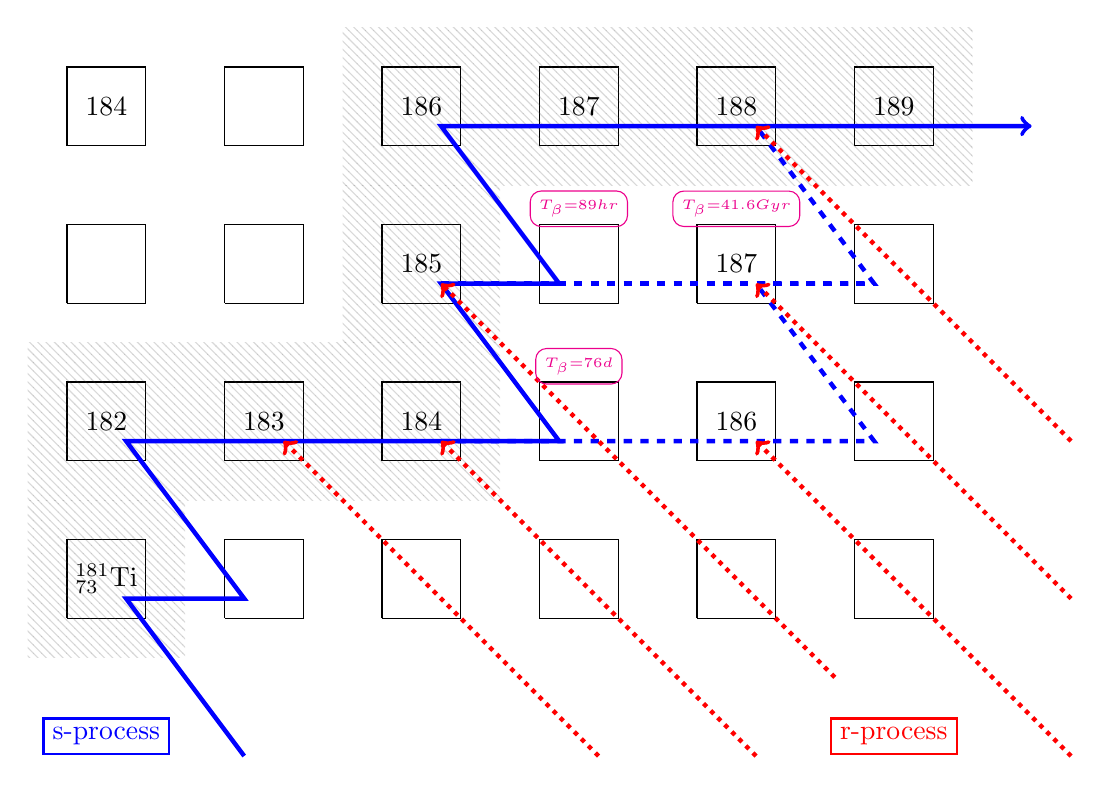
\begin{tikzpicture}
  %test in the middle
  %\draw (0,0) node {${}^{A+1}_{Z}$X};
  %\tikzsquare{0}{0}{\halfwidthnuclides}
  %Os-row on top of test
  \iffalse %old version
  \draw (-\distancenuclides,\distancenuclides) node {${}^{186}_{76}$Os};
  \tikzsquare{-\distancenuclides}{\distancenuclides}{\halfwidthnuclides}
  \draw (0,\distancenuclides) node {${}^{187}_{76}$Os};
  \tikzsquare{0}{\distancenuclides}{\halfwidthnuclides}
  \draw (\distancenuclides,\distancenuclides) node {${}^{188}_{76}$Os};
  \tikzsquare{\distancenuclides}{\distancenuclides}{\halfwidthnuclides}
  %stable Re-isotopes
  \draw (-\distancenuclides,0) node {${}^{185}_{75}$Re};
  \tikzsquare{-\distancenuclides}{0}{\halfwidthnuclides}
  \draw (\distancenuclides,0) node {${}^{187}_{75}$Re};
  \tikzsquare{\distancenuclides}{0}{\halfwidthnuclides}
  %W island of stability
  \draw (\distancenuclides,-\distancenuclides) node {${}^{186}_{74}$W};
  \tikzsquare{\distancenuclides}{-\distancenuclides}{\halfwidthnuclides}
  %shaded region of stability
  \fill[color=lightgray,opacity=0.1, pattern=north west lines, pattern color=darkgray]
  (-0.5\distancenuclides,-0.5\distancenuclides)
  rectangle (-1.5\distancenuclides,1.5\distancenuclides)
  rectangle (1.5\distancenuclides,0.5\distancenuclides)
  rectangle (0.5\distancenuclides,-1.5\distancenuclides);
  \fi

  %draw stable nuclei from clayton64 fig.1.
  %row1 - Os-184, blank, Os-186, Os-187, Os-188, Os-189
  \drawnuclide{-3\distancenuclides}{\distancenuclides}{\halfwidthnuclides}{\os{184}};
  \drawsquare{-2\distancenuclides}{\distancenuclides}{\halfwidthnuclides};
  \drawnuclide{-\distancenuclides}{\distancenuclides}{\halfwidthnuclides}{\os{186}};
  \drawnuclide{0}{\distancenuclides}{\halfwidthnuclides}{\os{187}};
  \drawnuclide{\distancenuclides}{\distancenuclides}{\halfwidthnuclides}{\os{188}};
  \drawnuclide{2\distancenuclides}{\distancenuclides}{\halfwidthnuclides}{\os{189}};
  %row2 - blank, blank, Re-185, blank, Re-187, blank
  \drawsquare{-3\distancenuclides}{0}{\halfwidthnuclides};
  \drawsquare{-2\distancenuclides}{0}{\halfwidthnuclides};
  \drawnuclide{-\distancenuclides}{0}{\halfwidthnuclides}{\re{185}};
  \drawsquare{0}{0}{\halfwidthnuclides};
  \drawnuclide{\distancenuclides}{0}{\halfwidthnuclides}{\re{187}};
  \drawsquare{2\distancenuclides}{0}{\halfwidthnuclides};
  %row3 - W-182, W-183, W-184, blank, W-186, blank
  \drawnuclide{-3\distancenuclides}{-\distancenuclides}{\halfwidthnuclides}{\w{182}};
  \drawnuclide{-2\distancenuclides}{-\distancenuclides}{\halfwidthnuclides}{\w{183}};
  \drawnuclide{-\distancenuclides}{-\distancenuclides}{\halfwidthnuclides}{\w{184}};
  \drawsquare{0}{-\distancenuclides}{\halfwidthnuclides};
  \drawnuclide{\distancenuclides}{-\distancenuclides}{\halfwidthnuclides}{\w{186}};
  \drawsquare{2\distancenuclides}{-\distancenuclides}{\halfwidthnuclides};
  %row4 - Ta-181, blank, blank, blank, blank, blank
  \drawnuclide{-3\distancenuclides}{-2\distancenuclides}{\halfwidthnuclides}{${}^{181}_{73}$Ti};
  \drawsquare{-2\distancenuclides}{-2\distancenuclides}{\halfwidthnuclides};
  \drawsquare{-\distancenuclides}{-2\distancenuclides}{\halfwidthnuclides};
  \drawsquare{0}{-2\distancenuclides}{\halfwidthnuclides};
  \drawsquare{\distancenuclides}{-2\distancenuclides}{\halfwidthnuclides};
  \drawsquare{2\distancenuclides}{-2\distancenuclides}{\halfwidthnuclides};

  %shaded region of stability
  \fillrectangle{-3\distancenuclides}{-2\distancenuclides}{2\halfwidthnuclides}; %Ta-181
  \fillrectangle{-3\distancenuclides}{-\distancenuclides}{2\halfwidthnuclides}; %W-182
  \fillrectangle{-2\distancenuclides}{-\distancenuclides}{2\halfwidthnuclides}; %W-183
  \fillrectangle{-\distancenuclides}{-\distancenuclides}{2\halfwidthnuclides}; %W-184
  \fillrectangle{-\distancenuclides}{0}{2\halfwidthnuclides}; %Re-185
  \fillrectangle{-\distancenuclides}{\distancenuclides}{2\halfwidthnuclides}; %Os-186
  \fillrectangle{0}{\distancenuclides}{2\halfwidthnuclides}; %Os-187
  \fillrectangle{\distancenuclides}{\distancenuclides}{2\halfwidthnuclides}; %Os-188
  \fillrectangle{2\distancenuclides}{\distancenuclides}{2\halfwidthnuclides}; %Os-189
  %\fillrectangle{\distancenuclides}{0}{2\halfwidthnuclides}; %Re-187
  %\fillrectangle{\distancenuclides}{-\distancenuclides}{2\halfwidthnuclides}; %W-186

  %draw s-process path
  \draw [ultra thick, ->, blue] (-2\distancenuclides-\offset,-3\distancenuclides-\offset)
  -- (-3\distancenuclides+\offset,-2\distancenuclides-\offset) -- (-2\distancenuclides-\offset,-2\distancenuclides-\offset)
  -- (-3\distancenuclides+\offset,-\distancenuclides-\offset) -- (0-\offset,-\distancenuclides-\offset)
  -- (-\distancenuclides+\offset,0-\offset) -- (0-\offset,0-\offset)
  -- (-\distancenuclides+\offset,\distancenuclides-\offset) -- (3\distancenuclides-\offset,\distancenuclides-\offset);
  %draw s-process branching point
  \draw [ultra thick, dashed, blue] (-\distancenuclides+\offset,-\distancenuclides-\offset)
  -- (2\distancenuclides-\offset,-\distancenuclides-\offset) -- (\distancenuclides+\offset,0-\offset)
  -- (2\distancenuclides-\offset,0-\offset) -- (\distancenuclides+\offset,\distancenuclides-\offset);
  \draw [ultra thick, dashed, blue] (-\distancenuclides+\offset,0-\offset)
  -- (2\distancenuclides-\offset,0-\offset);

  %draw r-process paths
  \draw [ultra thick, dotted, ->, red] (0+\offset,-3\distancenuclides-\offset)
  -- (-2\distancenuclides+\offset,-\distancenuclides-\offset);
  \draw [ultra thick, dotted, ->, red] (\distancenuclides+\offset,-3\distancenuclides-\offset)
  -- (-\distancenuclides+\offset,-\distancenuclides-\offset);
  \draw [ultra thick, dotted, ->, red] (1.5\distancenuclides+\offset,-2.5\distancenuclides-\offset)
  -- (-\distancenuclides+\offset,0-\offset);
  \draw [ultra thick, dotted, ->, red] (3\distancenuclides+\offset,-3\distancenuclides-\offset)
  -- (\distancenuclides+\offset,-\distancenuclides-\offset);
  \draw [ultra thick, dotted, ->, red] (3\distancenuclides+\offset,-2\distancenuclides-\offset)
  -- (\distancenuclides+\offset,0-\offset);
  \draw [ultra thick, dotted, ->, red] (3\distancenuclides+\offset,-\distancenuclides-\offset)
  -- (\distancenuclides+\offset,\distancenuclides-\offset);

  %add text
  \addtolength\offset{1.8\offset}
  \draw (-3\distancenuclides, -3\distancenuclides) node[thick, draw, blue] {s-process};
  \draw (2\distancenuclides, -3\distancenuclides) node[thick, draw, red] {r-process};
  \draw (0,0+\offset) node[draw=magenta, magenta, rounded corners] {${\scriptscriptstyle T_{\beta}=89hr}$}; %halflife of Re-186
  \draw (0,-\distancenuclides+\offset) node[draw=magenta, magenta, rounded corners] {${\scriptscriptstyle T_{\beta}=76d}$}; %halflife of W-185
  \draw (\distancenuclides,0+\offset) node[draw=magenta, magenta, rounded corners] {${\scriptscriptstyle T_{\beta}=41.6Gyr}$}; %halflife of Re-187
  \addtolength\offset{-1.8\offset}
\end{tikzpicture}
\caption[Chart of nuclides from \mycitetwo{clayton64}{fig.1} around A=187]{\label{tikz:nuclide-chart}
  Chart of nuclides around massnumber 187, adopted from \mycitetwo{clayton64}{fig.1}.
  The stable nuclei are denoted with their chemical symbols.
  The path of the s-process follows the valley of stability (shaded region), and is drawn as a blue solid line.
  Neutrons are absorbed during the s-process until and unstable isotope is reached, the unstable nuclide then \betadecay{s} to the higher isobars\footnote{the highest stable isobar means the nuclei with the same amount of nucleons and the highest amount of protons}.
  R-process nuclei are already very neutron-rich, and \betadecay{s} to the highest stable isobar.
  The path of the r-process is shown as red dotted lines.
  \w{185}, and also \re{186}, are potential branching points (), and can cause branched s-proces paths that are shown as blue dashed lines.
  The half-lifes of these potential branching point nuclei, as well as the half-life of \re{187}, are written in magenta over the nuclei.
}

%% \end{figure}


From the chart on can see the usual path for slow neutron capture along the valley of stability.
This is the main contribution to \os{187}. In a standard s-process analysis, \w{185} and \re{186} are unstable, and will decay before they can capture neutrons. The s-process path will never synthesize \re{187}. However if the neutron capture rate is comparable to the \betadecay rates of those nuclides a branching point can occur. A branching point is a point where the synthesizing path of the s-process split due to competing nuclear reactions. In this case a significant fraction of the s-process path can go through \re{186} to \re{187} or through \w{185} to \w{186} (which is stable) and onwards to \re{187}. Apart from these effects \re{187} is shielded from s-process contribution.

The rapid neutron capture maintains very high neutron numbers until the neutron source ``shuts off'', at that point the isotopes \betadecay to the valley of stability. Given the long \halflife of \re{187} it can be considered stable, so the \os{187} isotope is shielded from r-process contribution because almost all \betadecay on the 187-isobar will stop at \re{187}.

Since \re{187} is radioactive with a halflife of \comment{add here} some \re{187} in the interstellar or stellar medium will decay to \os{187}. This amount is called the cosmoradiogenic \os{187}. The fraction between cosmoradiogenic \os{187} and current \re{187} is given by the exponential decay-function (assuming ofcourse that the nuclear decay rate is constant for all time, including stellar environments), meaning the time of nucleosynthesis can be calculated from the observed fraction of daughter-parent nuclei.

Clayton attempts to calculate the fraction of cosmoradiogenic osmium and the age of nucleosynthesis from these principles\mycite{clayton64}.
A brief summary follows:

The abundance of \os{186} is due to s-process only, and the abundance of \os{187} is due to s-process (from \os{186}) and cosmo radiogenic enrichment from \re{187} beta-decay.
The s-process contribution from \os{186} is given by the \os{186} abundance and the ratio between the cross-section of the isotopes. It is shown from nebular Samarium that the two s-only isotopes have nearly identical cross-section times abundance. Extrapolating this to other s-process isotopes, the result is:
(denoting abundance of isotope by their chemical name instead of N for simplicity)
\begin{equation}
  \bar{\sigma}_{\os{186}}{\os{186}} = \bar{\sigma}_{\os{187}}{\os{186}_S}
  \quad \rightarrow \quad
  {\os{186}_S} = \frac{\bar{\sigma}_{\os{186}}}{\bar{\sigma}_{\os{187}}}{\os{186}}
\end{equation}
$\bar{\sigma}$ are the neutron-capture cross-sections averaged over the appropriate thermal velocity distributions.
The cosmoradiogenic component of \os{187} is therefor the remaining part.
\begin{equation}
  \os{187}_c = \os{187} - \os{187}_s = \os{187} - \frac{\bar{\sigma}_{\os{186}}}{\bar{\sigma}_{\os{187}}}{\os{186}}
\end{equation}
Rewriting equation to relative units.
\begin{equation}
  \frac{\os{187}_c}{\re{187}} = \frac{\os{187} - \frac{\bar{\sigma}_{\os{186}}}{\bar{\sigma}_{\os{187}}}{\os{186}}}{\re{187}} =
  \frac{
    \left(\frac{\os{187}}{Os}\right) -
    \frac{\bar{\sigma}_{\os{186}}}{\bar{\sigma}_{\os{187}}}
    \left(\frac{\os{186}}{Os}\right)
  }{
    \left(\frac{\re{187}}{Re}\right)
  }
  \left(\frac{Os}{Re}\right)
\end{equation}
Origin of time, t=0, is set to \sos formation. Assuming that r-process events are supernovae and they began occuring at time T before \sos formation(t=0), and the frequency of events decreases exponentially as $f_0e^{\Lambda t}$, where $f_0$ is the initial supernovae freqency.
According to this model, and Clayton, the amount of cosmoradiogenic \os{187} is given by
\begin{equation}
  \frac{\os{187}_c}{\re{187}} = \left[
    \frac{\Lambda-\lambda}{\Lambda}
    e^{\lambda T}
    \frac{1-e^{-\Lambda T}}{1-e^{-(\Lambda-\lambda) T}}
    \right] - 1
\end{equation}
And the two special cases. \\
Sudden synthesis ($\Lambda\rightarrow\infty$)
\begin{equation}
  \frac{\os{187}_c}{\re{187}} = e^{\lambda t} - 1
\end{equation}
Uniform synthesis ($\Lambda\rightarrow 0$)
\begin{equation}
  \frac{\os{187}_c}{\re{187}} = \frac{\lambda T}{1-e^{-\lambda t}} - 1
\end{equation}

\comment{end of direct summary}

In short, by modelling r-process nucleosynthesis and s-process nucleosynthesis, the fraction of \re{187}-\os{187} in the \sos can predict the time of nucleosynthesis from non-cosmological methods.
\comment{\\ What do I mean about the age of nucleosynthesis?}
\fi
